\documentclass[11pt]{article} 
\def\names{Hunter Kruger-Ilingworth (14198489)\\ 
Quentin Bouet (14198423) \\
Thomas Mehes (14259613) \\}
\def\doctitle{Assignment 2 \\ \note{Dew Point Generator Controller and Sensor Data Logger}}
\def\subjectcode{CC3501}
% Geometry and Layout
    \usepackage[margin=0.75in]{geometry}
    \usepackage{multicol}

% Graphics and Diagrams
    \usepackage{xcolor}
    \usepackage{graphicx} % Required for inserting images
    \usepackage[american]{circuitikz}
    \usepackage{tikz}
    \usepackage{tikz-3dplot}
    \usetikzlibrary{arrows.meta}
    \usepackage{pgfplots}
    \pgfplotsset{compat=newest}
    \usepackage{listings}
    \usepackage{tcolorbox}

% CSV Table input
    \usepackage{csvsimple, booktabs}

% Code Chunk Formatting
    \definecolor{comment_color}{rgb}{0.52,0.38,0.78}
    \definecolor{keyword_color}{rgb}{0.84,0.27,0.3}
    \definecolor{background_color}{rgb}{0.95,0.95,0.95}
    \usepackage{inconsolata} % Consolas-style font from the inconsolata package

\lstset{
    backgroundcolor=\color{background_color},   % Choose the background color
    commentstyle=\color{comment_color},       % Style of comments
    keywordstyle=\color{keyword_color},        % Style of keywords
    stringstyle=\color{red},              % Style of strings, assuming red
    basicstyle=\footnotesize\ttfamily, % Set font size, monospaced font, and color        
    breakatwhitespace=false,              % Automatic line breaking only at whitespace
    breaklines=true,                      % Automatic line breaking
    captionpos=t,                         % Caption position is on top
    keepspaces=true,                      % Keeps spaces in text
    numbers=left,                         % Line number position
    numbersep=5pt,                        % How far the line numbers are from the code
    showspaces=false,                     % Show spaces in the code
    showstringspaces=false,               % Underline spaces within strings only
    showtabs=false,                       % Show tabs within strings adding particular underscores
    tabsize=2,                            % Sets default tab size
    title=\lstname                        % Show the filename of files included with \lstinputlisting
}
% Text Content / Math
    \usepackage{lipsum} % Dummy text
    \usepackage{hyperref}
    \usepackage{amsmath} % For sum symbol and other math formatting

% Headers and Footers
    \usepackage{lastpage}
    \usepackage{fancyhdr}
    \makeatletter
    \renewcommand{\@seccntformat}[1]{}
    \makeatother
    \pagestyle{fancy}
    \fancyhf{} 
    \setlength{\headheight}{15pt}
    \fancyhead[L]{\subjectcode{} - \doctitle{}}
    \fancyhead[R]{} % Rearrange as you please
    \fancyfoot[L]{\name{}}
    \fancyfoot[R]{Page \thepage\ of \pageref{LastPage}} 
    \renewcommand{\headrulewidth}{0pt}

% Caption and Referencing Customization
    \usepackage{caption}
    \usepackage{cleveref}
    \DeclareCaptionLabelSeparator{IEEE}{.\quad }
    \captionsetup[figure]{name=Fig., labelsep=IEEE}
    \captionsetup{format=hang, labelfont=bf}
    \captionsetup{justification=raggedright,singlelinecheck=false}

% Document Metadata and First Page Formatting
    \title{\doctitle{}\\\large{James Cook University Cairns}}
    \author{\name{} (\studentnumber{})\\ 
    Quentin Boet (\note{whatever your number is }) \\
    Thomas Mehes (\note{whatever your number is }) \\}
    \date{\today}

% References
    \usepackage{natbib}


%Choose which files are re-rendered (saves rendering time)
%\includeonly{}

\newcommand{\insertimage}[3]{
\begin{figure}[h]
    \centering
    \includegraphics[width=\linewidth]{#1} % Image filename
    \caption{#2} % Caption
    \label{#3} % Label
\end{figure}
}

\newcommand{\insertbigimage}[3]{
\begin{figure*}[h]
    \centering
    \includegraphics[width=\linewidth]{#1} % Image filename
    \caption{#2} 
    \label{#3} 
\end{figure*}
}

\newcommand{\codeblock}[4]{
    \lstinputlisting[language=#1, caption={#2}, label=#3]{#4}
}


\newcommand{\E}[1]{
    \cdot 10^{#1}
}

\newcommand{\abs}[1]{
    \left\lvert #1 \right\rvert
}

\newcommand{\note}[1]{\textcolor{red}{#1}} %create a note for yourself


\definecolor{codegray}{gray}{0.9} % Light gray color
\newcommand{\code}[1]{\colorbox{codegray}{\texttt{\detokenize{#1}}}} % Command for inline code

\begin{document}
    % Create the title page
    \begin{titlepage}
        \maketitle
        \thispagestyle{empty} %suppresses page numbering on the title page
    \end{titlepage}

    % Table of Contents
    \thispagestyle{empty} % Suppresses page numbering on the contents page
    \onecolumn
    \tableofcontents
    \listoffigures
    \listoftables

    % Document - place new files as needed
    \clearpage
    \section{Intro}

This report details the design and implementation of an embedded system functioning as both a scientific data logger and a smart interface with an analogue dew point generator. Utilizing the RP2040 microcontroller, SDI-12 environmental sensors, and a load cell, the system collects and processes data for climate modelling. The project aims to offer a reliable and efficient solution for monitoring and controlling environmental parameters, especially in researching tropical plant behavior under varying climate conditions.

The LI-610 Dew Point Generator is a precision instrument that produces a stable gas stream with a controlled dew point. It employs Peltier thermoelectric coolers to regulate water reservoir temperatures, ensuring the air stream is fully saturated with water vapor. This precise dew point control is vital in environmental research, preventing condensation in climate-controlled chambers and maintaining experimental conditions and data accuracy.

Accurate, continuous monitoring of environmental parameters is crucial for tropical plant research, but traditional methods are labor-intensive, error-prone, and physical presence in climate-controlled rooms can disrupt experiments. Commercial solutions like Campbell Scientific are often expensive and closed-source, limiting accessibility and customization for researchers. This project provides an open-source, cost-effective alternative for remote monitoring and control. By integrating various sensors and a smart interface for the dew point generator, the system enables the simulation of different climate conditions and monitoring of plant responses without entering the controlled environment, ensuring data integrity while enhancing flexibility and affordability.
    \insertbigimage{figures/block_diagram.pdf}{Block diagram of the system}{block_diagram}

\section{System Design Overview}

The system was designed around the RP2040 microcontroller, acting as the central 
processing unit for interfacing with a variety of sensors and control devices. 
The design incorporates the SF-5M sap flow sensor, LT-1T leaf temperature sensor, 
and MT-603 load cell to measure various environmental parameters. Each of these 
sensors use different communication protocols, requiring careful consideration of 
power requirements, signal integrity, and communication compatibility. \cref{block_diagram} 
shows an overview of all the communication systems involved in the design.

\begin{figure}
    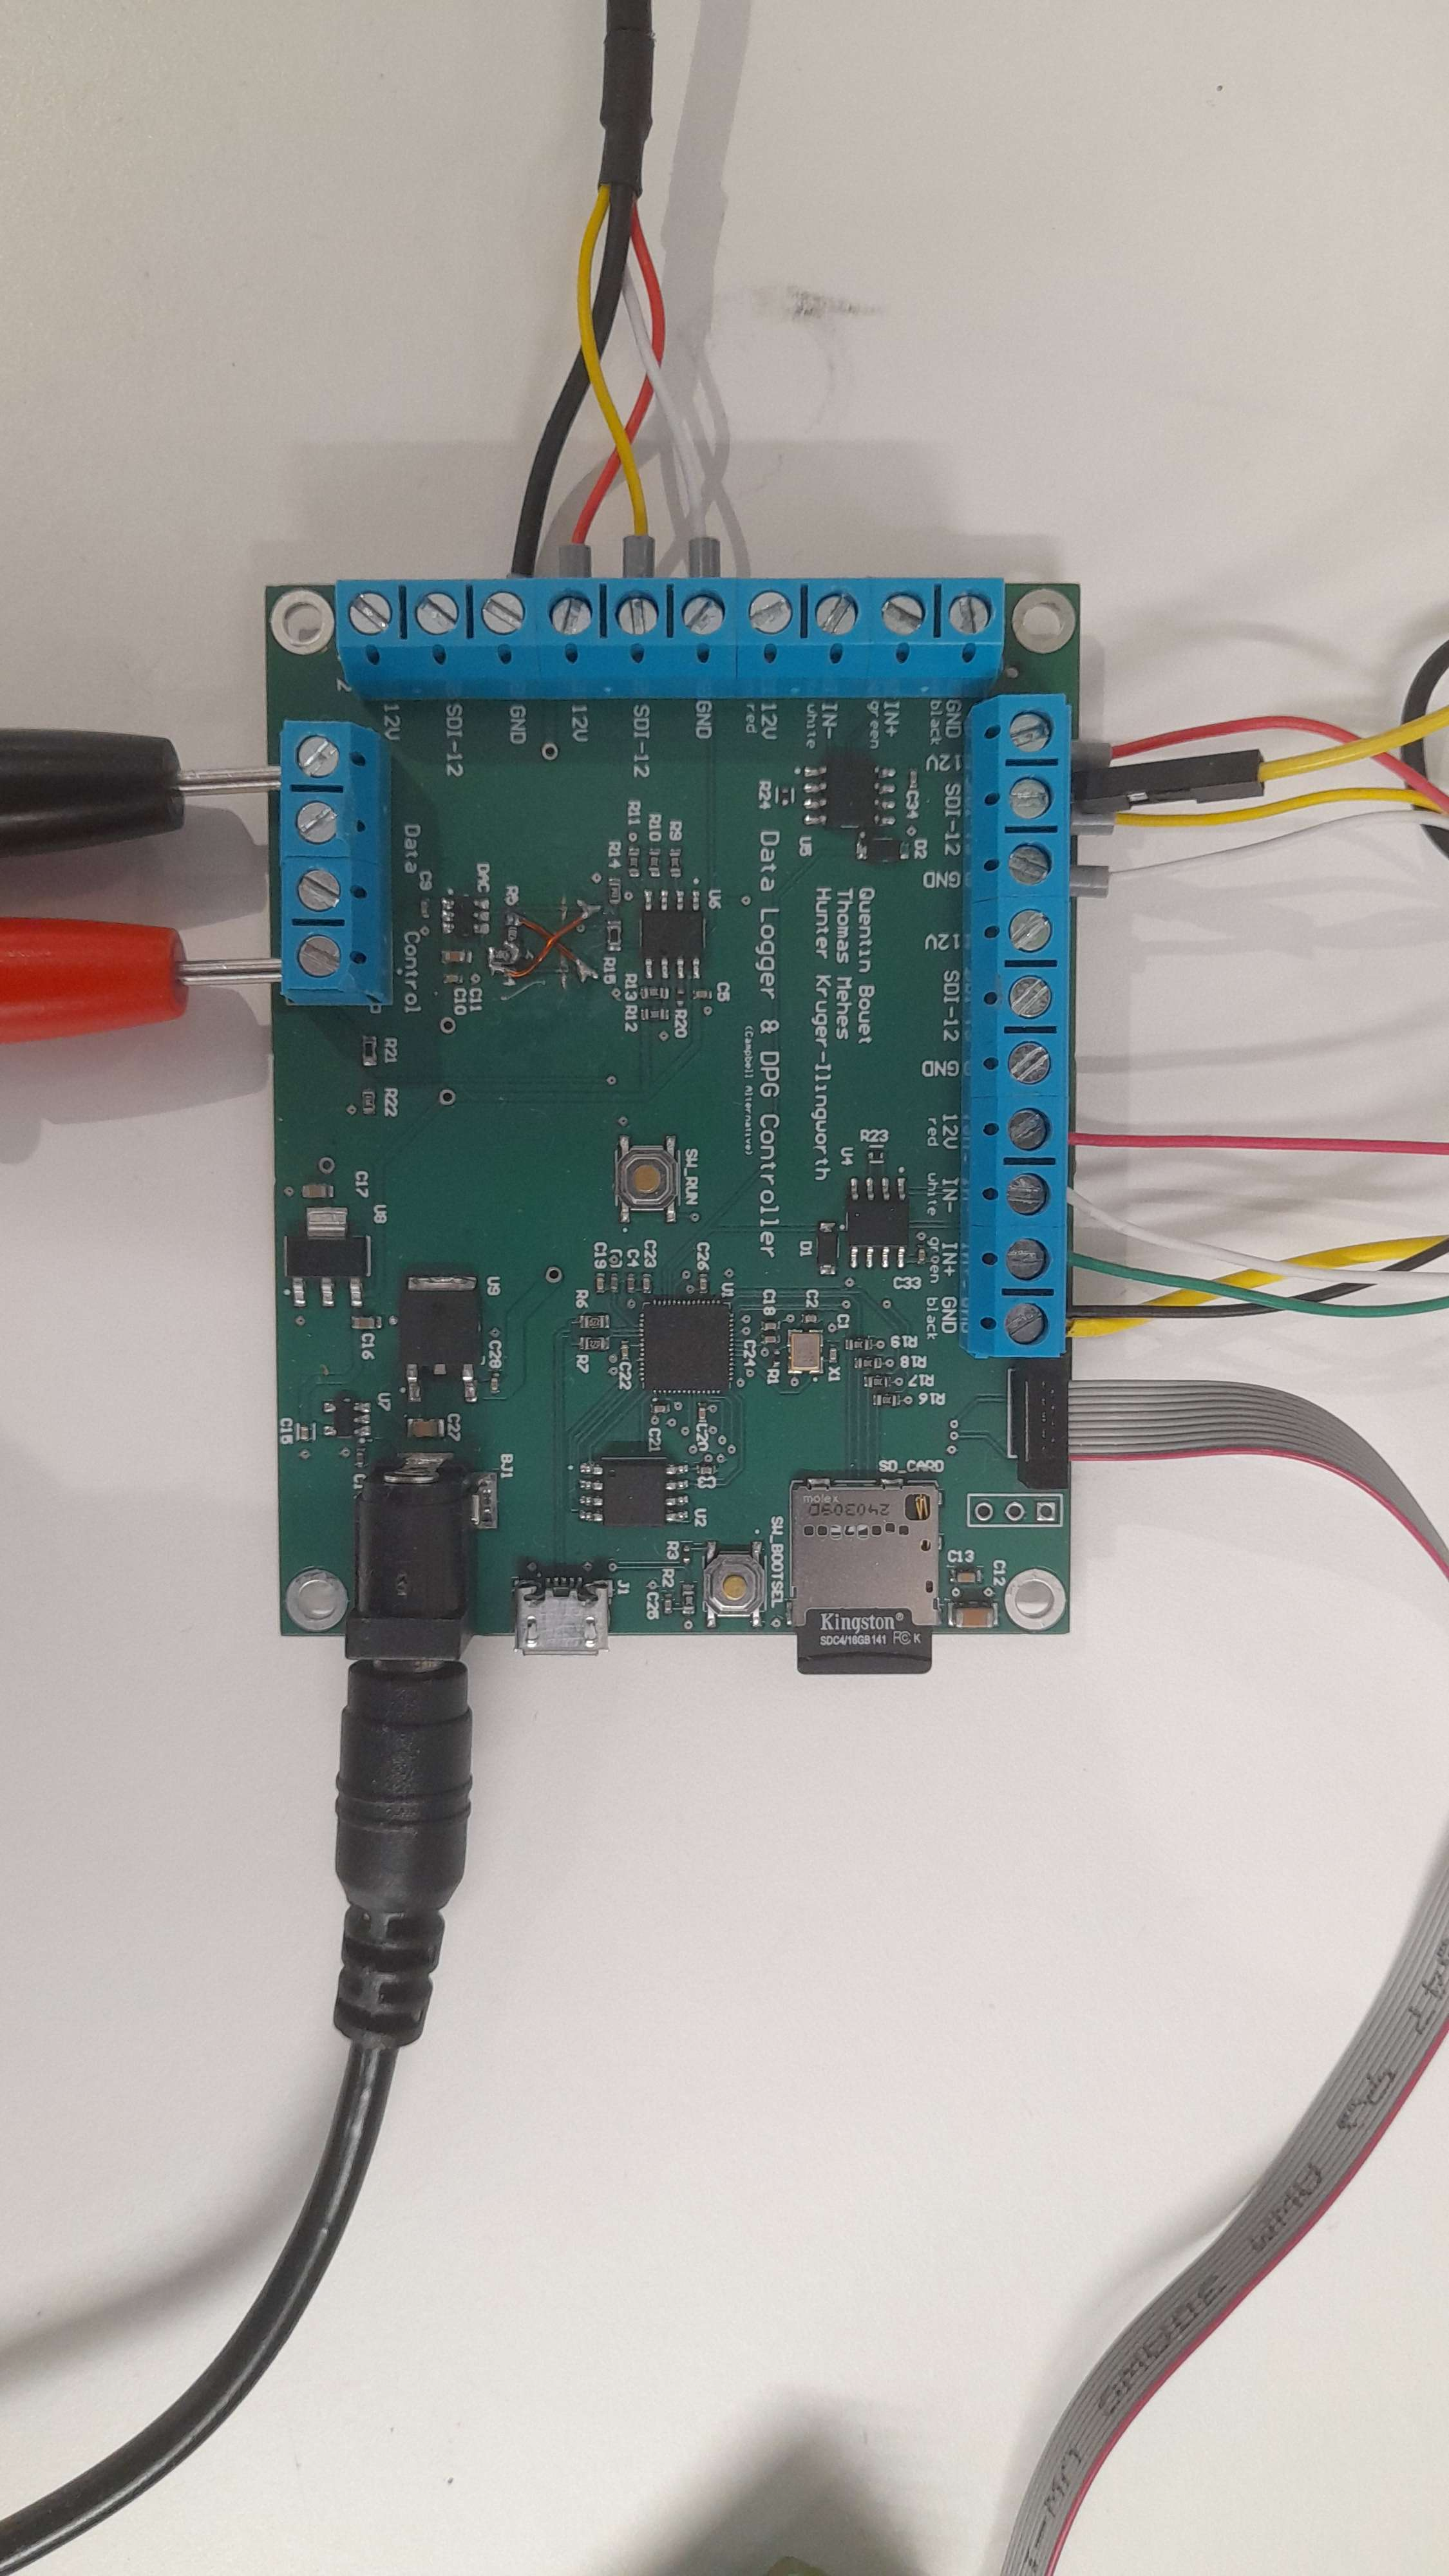
\includegraphics[width=0.4\linewidth]{figures/board_photo.jpg}
    \caption{Photo of Board}
    \label{board_photo}
\end{figure}

\begin{figure}
    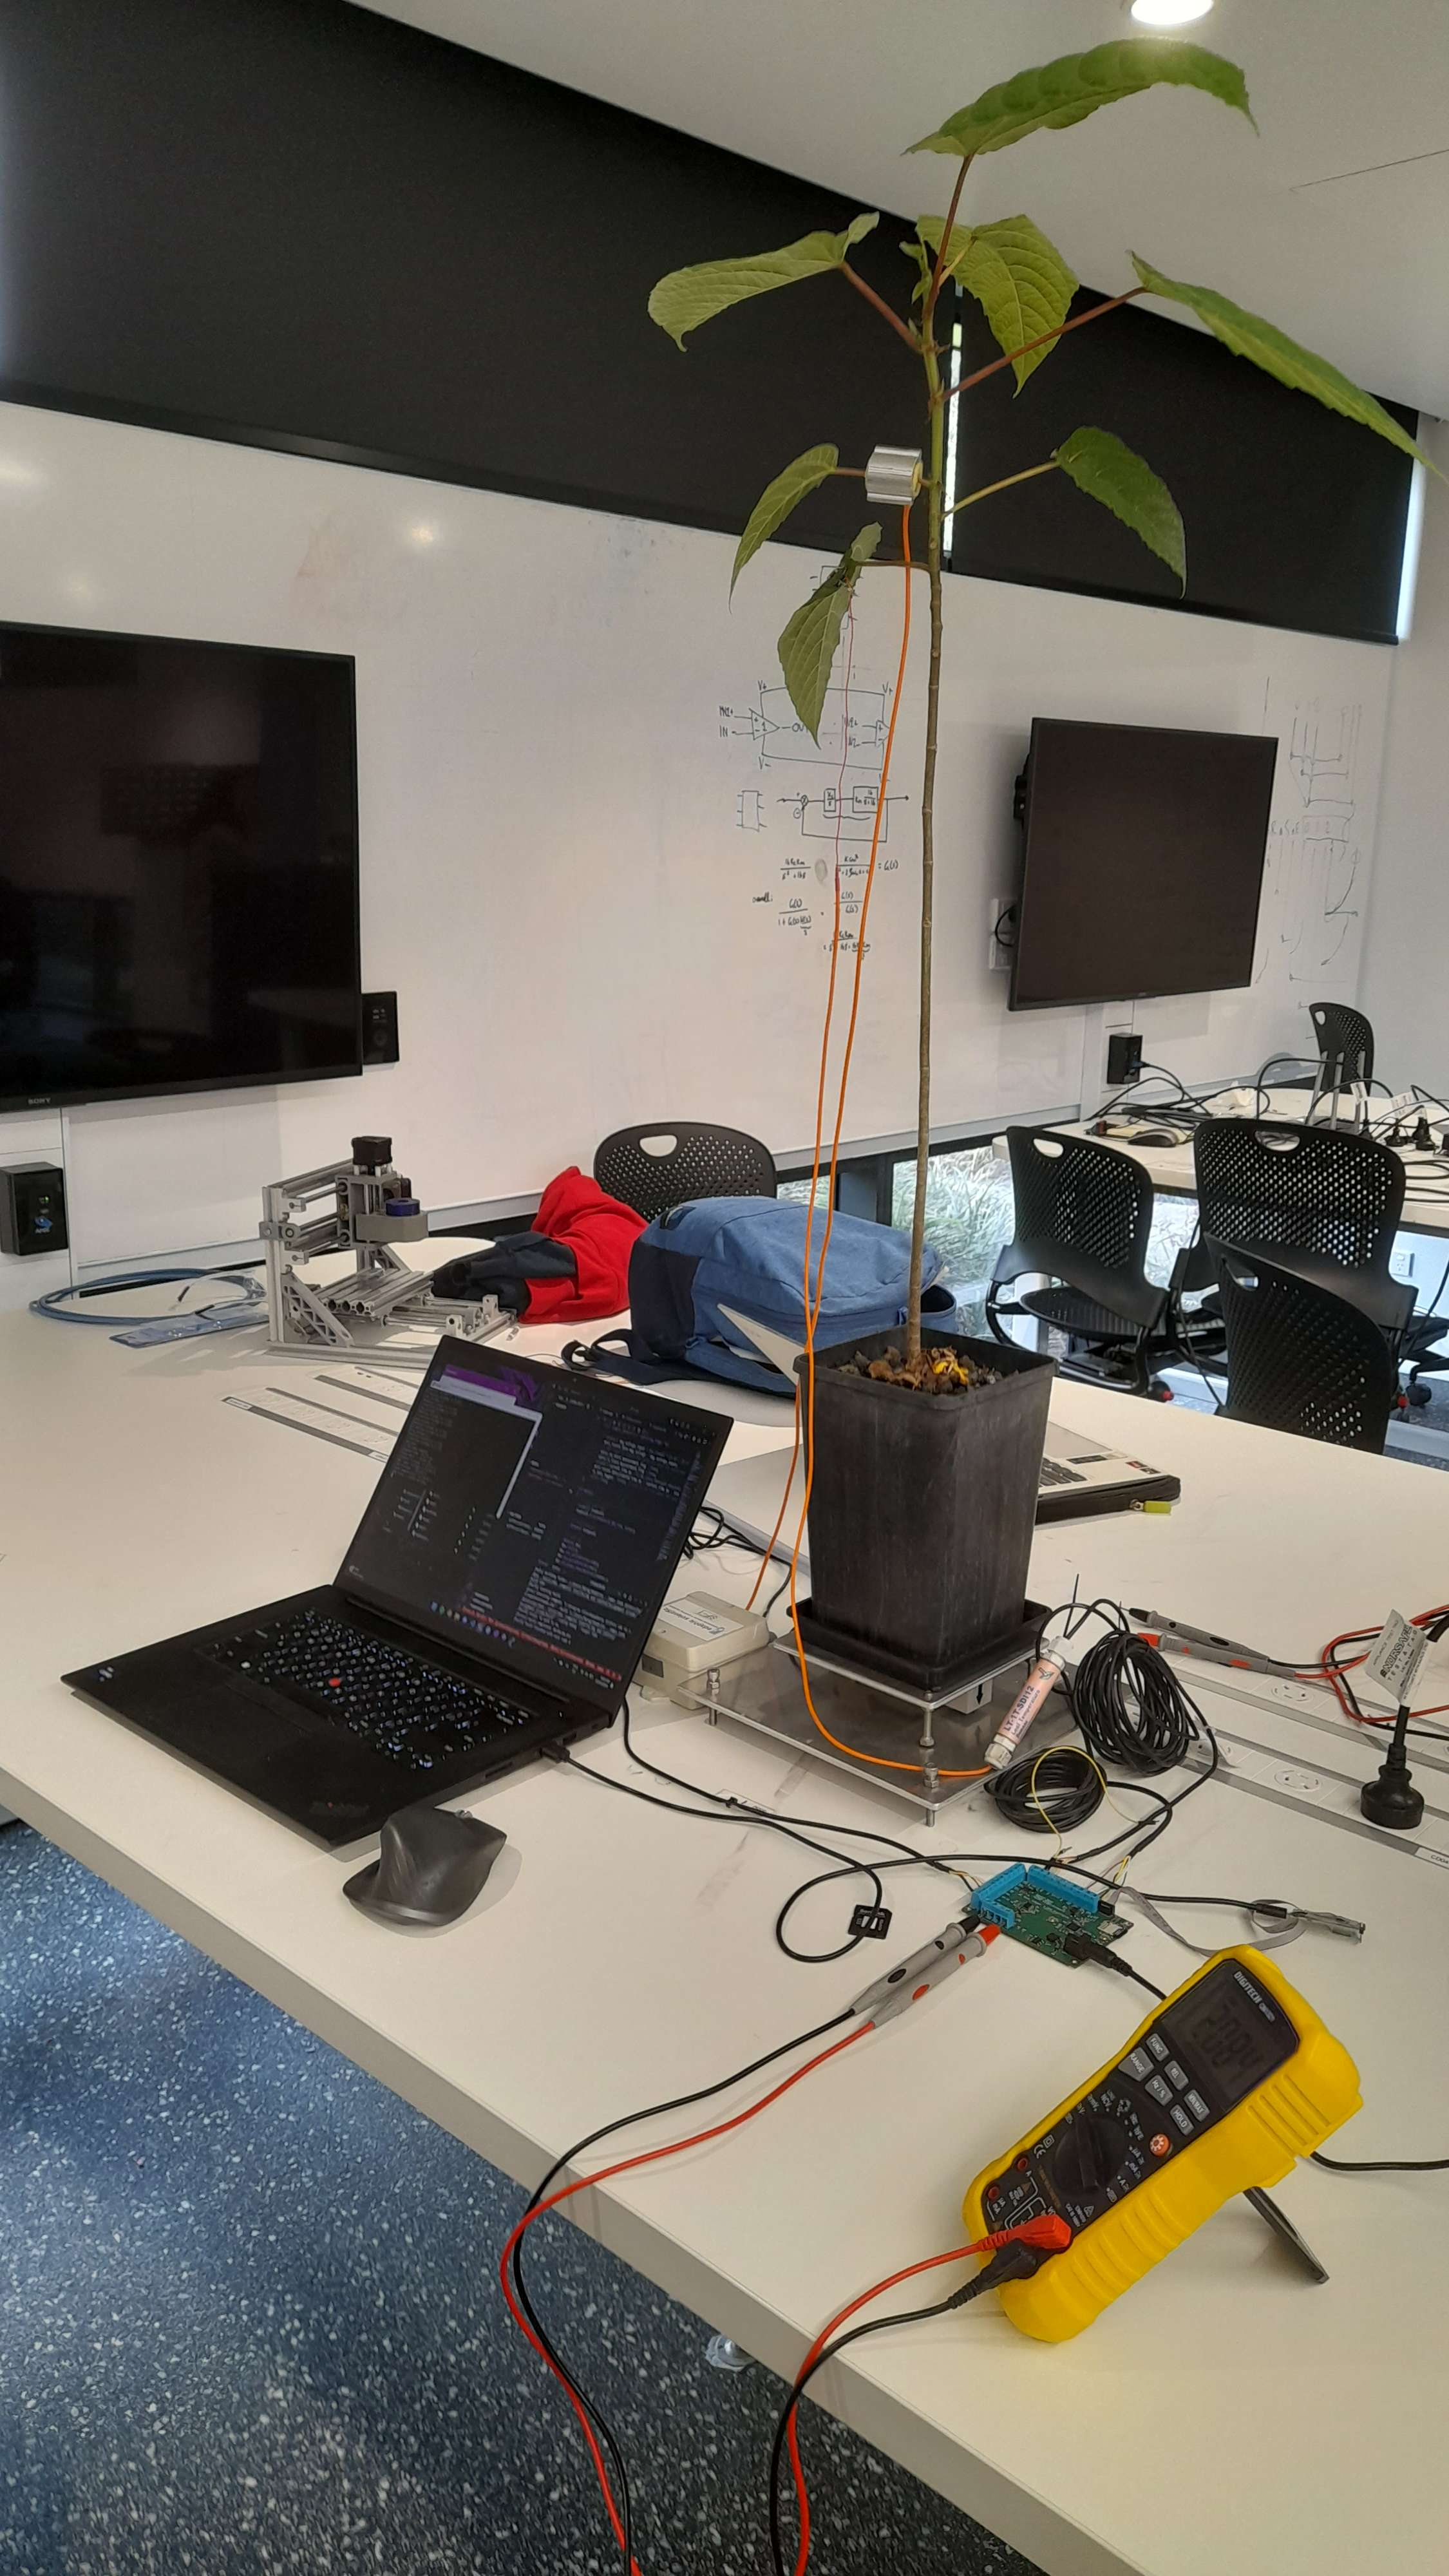
\includegraphics[width=0.4\linewidth]{figures/system_setup_1.jpg}
    \caption{Photo of System Setup}
    \label{system_photo}
\end{figure}


    \subsection{Components}

\note{Feel free to move and change the name of this subsection later}

This is my cool document. I have a lot of cool things to say. I was here. \note{note to self: Improve this introduction}

i can use citations too \cite{normal_distribution_wiki_page}.

\begin{figure}
    \begin{center}
    \begin{tikzpicture}[auto, node distance=2cm,>=latex']
        
        % Inputs
        % \node [input] (input_name) {};
        \node [input] (sensor_1) {};
        \node [input, yshift= 1cm] (sensor_2) {};
        \node [input, yshift= -1cm] (sensor_3) {};

        % Blocks
        % \node [block, location, node distance=xcm, minimum width=xcm] (block_name) {label};
        \node [block, right of=sensor_1, node distance=3cm, minimum width=2cm, minimum height=3cm] (RP2040) {RP2040};

        % Outputs
        % \node [output, location] (output_name) {};
        \node [output, right of=RP2040] (output) {};

        % Arrows
        % \draw [->] (point_A) -- node {label} (point_B);
        \draw [->] (sensor_1) -- ++ (2,0) node [near start, above] {load cell} (RP2040);
        \draw [->] (sensor_2) -- ++ (2,0) node [near start, above] {sap flow sensor} (RP2040);
        \draw [->] (sensor_3) -- ++ (2,0) node [near start, above] {leaf temp} (RP2040);

        \draw [->] (RP2040) -- node [near end, above] {output} (output);
            
    \end{tikzpicture}
    \end{center}
    \caption{Block of diagram of the system}
    \label{block_diagram}
\end{figure}

As seen in \cref{block_diagram} there were lots of blocks


SDI-12

\begin{figure}
    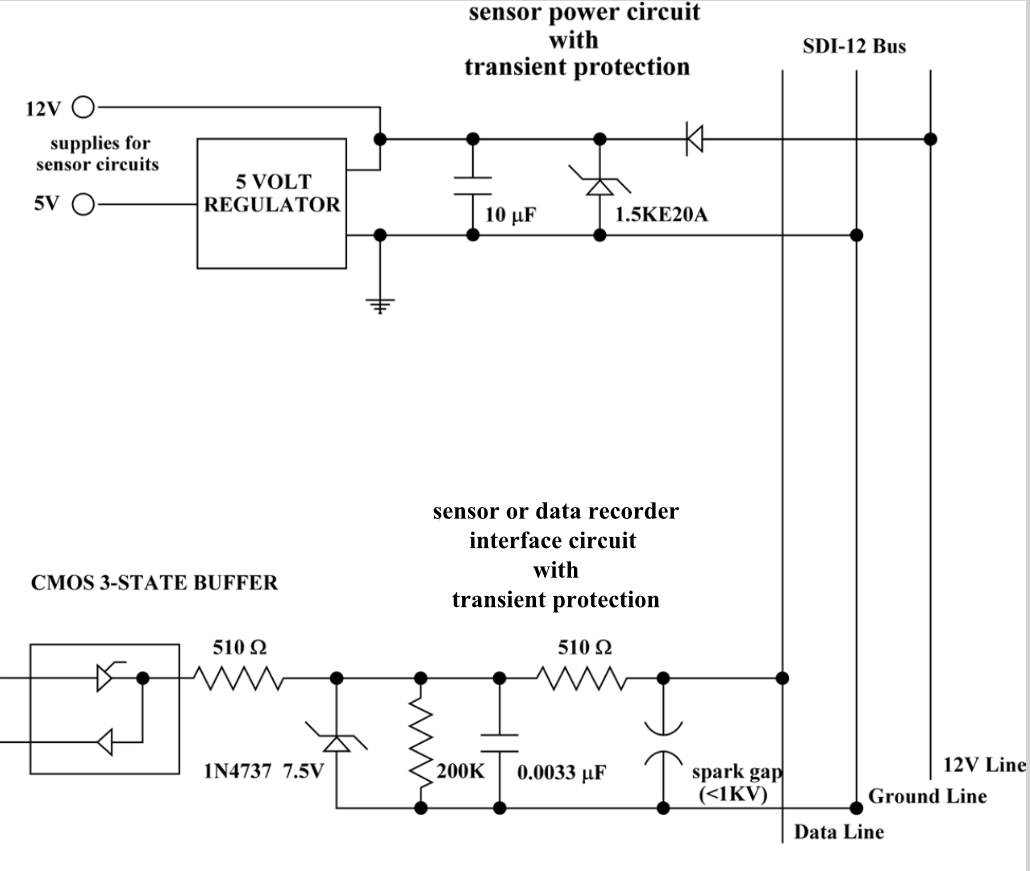
\includegraphics[width=\linewidth]{SDI-12 circuit.png}
    \caption{SDI-12 Circuit}
    \label{sdi12_circuit}
\end{figure}
    \section{Technical Challenges and Solutions}

\subsection{SDI-12 Sensor Communication Issues}
During the testing of the SDI-12 sensors, initial attempts to communicate using RS485 transceivers failed due to improper framing of byte streams. The strict timing requirements of the SDI-12 protocol made it difficult to achieve reliable communication using standard UART settings. This issue was addressed by applying the \code{uart_set_format()} function, which allowed the RP2040 to handle the SDI-12 protocol's timing more accurately. Additionally, a \code{custom is_timed_out()} function was created to automate character reception without using traditional sleep methods, ensuring precise byte timing and avoiding data loss during transmission.

\subsection{Load Cell Signal Scaling and Stability}
The MT-603 load cell exhibited a significant dead zone and provided inconsistent readings due to mechanical vibrations in the experimental setup. Software-based noise reduction techniques, such as averaging past data points, were implemented to mitigate the effect of oscillations. This software solution was preferred over hardware filtering due to the constraints of the existing apparatus.

\note{Issues with clk and data lines being connected the wrong way around on the RP2040}
    \section{Discussion}

\lipsum[1]

    \section{Conclusion}

\note{This section will summarize the project's outcomes, reflecting on the objectives achieved and providing final thoughts.}
    \section{Appendix}

\onecolumn
\codeblock{python}{Example Python Code}{code_example}{code/python.py}
%\codeblock{Matlab}{Example MATLAB Code}{code_example}{../code/main.m}
%if you're using the MATLAB report template


    \bibliographystyle{IEEEtranN} 
    \bibliography{references} 

\end{document}